\documentclass[12pt]{report}

\usepackage[hidelinks]{hyperref}
\usepackage{graphicx}
\usepackage{cite}

\title{Classroom Management Handbook}
\author{Lyron Winderbaum}

\begin{document}

\maketitle

\tableofcontents

\chapter{Introduction}

This document is written as a reference manual of strategies for classroom behaviour management. The goal is that a teacher could consult this document in order to prompt them on strategies they might have forgotten about or not thought of. The language used will be deliberately concise, and is not intended to be comprehensive --- quite the opposite, it is intended as a memory prompt, not an encylopedia.

This handbook is organised by chapters. Chapters \ref{chap:preventative}, \ref{chap:supportive} and \ref{chap:corrective} introduce a list of strategies, each as a section or sub-section.
Again this list is not intended to be comprehensive, but rather represents a selection of strategies that resonate with me personally. These chapters seperate strategies into the three broad categories of \cite{Charles2002}: preventative, supportive, and corrective, respectively. In the interests of brevity I will keep the descriptions of these strategies minimal, only providing examples and further elaboration in later chapters and appendices. Chapter \ref{chap:video_examples} discusses some of the videos shown in lectures in the context of these strategies, providing some examples of their use in practice. Finally, Chapter \ref{chap:theories} discusses some popular theorists, and how the theory relates to the strategies.

\textbf{Disclaimer 1:} I've written this document from my perspective, so any statements that are not explicitly referenced to be otherwise are my personal oppinion and nothing more.

\textbf{Disclaimer 2:} In some places I might use language such as "It is wrong to...", "You should...", etc. --- it is important to recognise that every situation comes with it's own intricacies and context and that no such absolute statements can ever be universal.










\chapter{Preventative Strategies}
\label{chap:preventative}

These are strategies that apply when there is no specific misbehaviour being addressed, but rather are preventative in the sense that they describe approaches that can help prevent problematic misbehaviour ever occuring in the first place. These are by far the most preferable strategies to be using and so should always be the place to start. Other strategies should only be attempted if the preventative strategies have already failed. 



\section{Praise}
\label{sec:praise_p}

Praise your students! Some students may never have been praised before, don't underestimate the power it can have. Be specific with your praise --- refer to something specific they have done, whether it be some work or their self-regulation, whatever. Most importantly: \textbf{be genuine}. Warning: if your praise is not genuine, your students will know, and they will not appreciate it.



\section{Don't Assume}
\label{sec:dont_assume_p}

You don't know what your students have gone through at home or in their lives. You don't know if their misbehaviour is malicious or is just coming from learnt emotional reactions they have no control over. \textbf{You don't know} --- don't assume. When confronted by misbehaviour, don't immediately react with criticism or condemnation --- instead, train your initial reflex reaction to be one of compassionate calm. Warning: If you make assumptions about a students misbehaviour, they will pick up on it and they will not appreciate it. Conversely, if you keep an open mind and focus on reacting compassionately, you could open the door to building rappor (\ref{sec:rapport_p}). This can also help in feeling genuine when giving praise (\ref{sec:praise_p}) and sympathy.

This strategy is obviously easier said than done, but it is an important one to keep in the back of your mind as you work on your personal development.



\section{Show Interest}
\label{sec:show_interest_p}

Be interested in what is going on in your students lives. This is a natural extension of not assuming and being compassionate (\ref{sec:dont_assume_p}), but can also lead to learning about what is important to your students and this can allow you to design relevant (\ref{sec:relevance_p}) and interesting (\ref{sec:fun_p}) lessons for them.



\section{Use Names}
\label{sec:use_names_p}

Learn the students names. Use them. Students will appreciate the effort you have gone too and the care for them you have demonstrated by doing so (\ref{sec:show_interest_p}). Similarly to praise (\ref{sec:praise_p}), the impact of this strategy is not to be underestimated.



\section{Rapport with Students}
\label{sec:rapport_p}

Praise (\ref{sec:praise_p}), using names (\ref{sec:use_names_p}) are both ways of showing interest (\ref{sec:show_interest_p}) in your students. When you do these things you can develop a rapport with the students that is a powerful, and valuble thing.



\section{Establish Routines and Procedures}
\label{sec:routines_p}

Habit is powerful. If you can instill routines into you class early, you can save yourself alot of headache in the future.

\subsection{Democratic setting of classroom practices}
\label{sec:democratic_setting_of_routines_p}

Discuss classroom practices with students --- give them an oppurtunity to share their oppinions. If they buy into the rules and routines by having influence on deciding what they are, they will have a sense of ownership, and be more likely to follow those rules and routines.



\section{Use of Language}
\label{sec:language_p}

The words we choose and the way we speak can have a profound impact on how people perceive us, and students can be particularly sensitive to this.

\begin{itemize}
  \item Use inclusive language --- don't assume (\ref{sec:dont_assume_p})!
  \item Use clear and concise sentences.
  \item Use appropriate vocabulary.
  \item Articulate well, and at an appropriate volume.
  \item If you have any English as an additional language students, or students with hearing impairments, ensure they have access to the information: 
  \begin{itemize}
    \item Use sign language (if possible), 
    \item Provide translations (if possible), 
    \item Speak slowly and clearly, 
    \item Articulate deliberately,
    \item Do the above without being condescending.
  \end{itemize}
\end{itemize}

\subsection{Clear Instructions}
\label{sec:clear_instructions_p}

It is particularly cruical to be clear when delivering instructions. For verbal instructions,
\begin{itemize}
  \item Be heard: Ensure there is silence before delivering instructions (same as \ref{sec:start_well_p}).
  \item Ensure students have access to all the information they need: If you are asking them to interpret an image, ensure they can see the image, etc. 
  \item Use clear verbs so it is clear what they are expected to do: "Draw", "Calculate", "Write", etc.
\end{itemize}

\subsection{Clear Materials}
\label{sec:clear_materials_p}

Delivering instructions clearly equally applies to written instructions, not only verbal instructions (\ref{sec:clear_instructions_p}). Appropriate (easy to read) fonts and vocabulary should be used for handouts, etc.



\section{Non-verbals}
\label{sec:non_verbals_p}

Similar to the use of language (\ref{sec:language}), non-verbals such as body language, positioning, attitude, facial expressions, etc. have a big impact on how you are perceived. 

\subsection{Enthusiasm}
\label{sec:enthusiasm_p}

The students can tell if you are genuinely enthusiastic about the lesson, about the topic, about seeing them, and enthusiasm is infectious.



\section{Preparation}
\label{sec:preparation_p}

This is an important strategy. If you put in work preparing for your classes, it will pay off both because the preparation itself, but also because your students will recognise the work you have put in for them, and appreciate it. 

\subsection{Relevance}
\label{sec:relevance_p}

Make material (lessons, activities, etc.) that is relevant to your students lives. If you ahve some rapport (\ref{sec:rapport_p}) with your students you can ask them what they are interested in and design lessons and activities around their interests.

\subsection{Fun}
\label{sec:fun_p}

Design interesting and fun lessons and activities! Similar to relevance (\ref{sec:relevance_p}) if you have some rapport (\ref{sec:rapport_p}) with your students you could try asking them what they think might be fun and try designing a lesson around that.

\subsection{Structure}
\label{sec:structure_p}

Design structured lessons. This is vague and broad, as it can be done in many ways, but having prepared an appropriate amount of activities and a structure linking them together in a lesson cannot be overstated in it's usefulness.



\section{Start Well}
\label{sec:start_well_p}

Before beggining a class, ensure that you have the classes' full attention, and complete silence. This is an important routine (\ref{sec:routines_p}) to set, in that if you can get your class into the routine of falling silent at the beggining of a class, it will make starting well much easier for you.

\subsection{Starter Activity}
\label{sec:starter_acivity_p}

A starter is a structured (\ref{sec:structure_p}) way to start a lesson, often it is a short (5-10min) activity that is fun, engaging, and easy, and serves the function of transitioning (\ref{sec:managing_transitions_p}) the students from being out of class or a in a different class to being in class, and in the appropriate mindset.




\section{Flow/ Momentum}
\label{sec:flow_p}

Once you have started well (\ref{sec:start_well_p}) and gotten the students engaged (see \ref{sec:relevance_p}, \ref{sec:fun_p}) you have gotten the momentum of the class started, then you need to maintain this "flow". This can be done by use of structure (\ref{sec:structure_p}) and managing transitions well (\ref{sec:managing_transitions_p}), but the exact process for doing this is difficult pin down because it is so context dependant. It involve a quality some refer to as "with-it-ness", which more or less is an awareness of the situation and the ability to see problems coming up before they occur and managing them before they derail the class --- this takes practice, and similar to "don't assume" (\ref{sec:dont_assume_p} is something to monitor and keep in the back of your mind as you work on your personal development as a teacher.

\subsection{Managing Transitions}
\label{sec:managing_transitions_p}

Starting well (\ref{sec:starting_well_p}) is a key example of making transitions, and it is a big one --- transitioning from outside the class to in the class. But there will be transitions inside the class as well from one activity to another, and these are the key points where momentum can easily be lost. To maintain good behaviour in your class being aware of these transitions before they occur, and having strategies in place to manage them in crucial. Similar to starting well (\ref{sec:starting_well_p}) and delivering clear instructions (\ref{sec:clear_instructions_p}) managing transitions well should start with ensuring quiet and complete attention before beggining the next activity, with an emphasis on making sure this finds its way into the classes routine (\ref{sec:routine}). 



\section{Mix different activities}
\label{sec:mix_differnt_activities_p}

If you do the same kind of activity over and over, it will get boring. Your students will get bored, and you don't want that. Mix it up! Use a variety of approaches and activities, some of them might not go well, but you can use that information to learn what works well with a particular group of students and what doesnt, and how to improve your preparation (\ref{sec:preparation_p}) in the future.



\section{Manage your time}
\label{sec:manage_your_time_p}

Time management is important. Reflect on how you have been spending your time in class --- have you been spending all your time speaking to the same students, are there some getting left behind? Have you been spending alot of time in class doing something that could be done beforehand (\ref{sec:preparation_p}), like writing on the whiteboard for example? Are these important?



\section{Model appropriate behaviors}
\label{sec:model_behaviours_p}

Don't be a hypocrite. Simple, if you are going to ask the students to behave a certain way --- adhere to the same standard yourself.


























\chapter{Supportive Strategies}
\label{chap:supportive}

These are for situations when the misbehavior is not so severe as to require being addressed directly. Instead, the students can be encouraged and guided via supportive strategies to adopt more productive and helpful behaviours.


\section{Praise}
\label{sec:praise_s}

Although praise can be preventative (\ref{sec:praise_p}), it can also be used as a supportive strategy. If you have students who sometimes meander off task, praising their on-task behaviour can encourage more on-task behaviours. Similarly, if you have attention seeking students, praising and giving your attention to other students who are on-task can encourage the attention seeking students to do on-task behaviours (depending on what was motivating their attention seeking behaviour to begin with --- if they were motivated by getting attention, then they might see others getting your attention by doing on-task behaviours and try to mimic that). 

\subsection{Acknowledge others good behaviour}
\label{sec:acknowledge_good_behaviour_s}

(VIDEO: Attention seeking students)


\section{Use Names}
\label{sec:use_names_s}

Similarly, using names can be preventative (\ref{sec:use_names_p}), but it can also be used as a supportive strategy. By using names when giving praise (\ref{sec:praise_s}) for example, you can reinforce that you are noticing a specific students on-task behaviour, strengthening that reinforcement by showing that you know their name and care enough to have remembered it.


\section{Show interest}
\label{sec:show_interest_s}

I don't remember why this was here...?

\section{Scaffolding}
\label{sec:scaffolding_s}

If students are losing interest and going off-task as a result of trying, but struggling to complete, a task perhaps due to it's difficulty or unfamiliarity to them, you can offer help in completing the task. While without aid their misbehaviour would likely only get worse, if you can give them a sense of success by helping them complete the task, you can then slowly ease back the amount of scaffolding (help) you provide them until they are able to do more and more of the task themselves. Often this will result in a feeling of accomplishment on their part, and will encourage on-task behaviour.

Note link to ZPD theory.


\section{Proximity ("The Whisper Technique")}
\label{sec:proximity_s}

Although proximity can be used to discourge misbehaviour, this is more of a corrective (\ref{sec:proximity_c}). Proximity can be used as a supportive strategy by using it to deliver help (\ref{sec:scaffolding_s}) privately. Often if you offer help publically (in front of the students classmates) it can be embarressing for them and they might not be receptive. In contrast, using proximity to deliver aid in a whisper that is not as public can improve the likelyhood of the scaffolding (\ref{sec:scaffolding_s}) to be successful.

\section{Eye Contact}
\label{sec:eye_contact_s}

\section{Tactical Ignoring}
\label{sec:tactical_ignoring_s}

This is borderline corrective, but as mentioned in \ref{sec:praise_s} one approach to dealing with attention seeking behaviours can be to "tactically ignore" the misbehaviour, instead focusing on and praising (\ref{sec:praise_s}) on-task behaviour elsewhere in the classroom. 

VIDEO REFERENCE: Attention seeking students. 

\section{Wait time.}
\label{sec:wait_time_s}


Broken Sentencees --- pause to get attention (VIDEO: Manage that lesson (chemistry year 8)

\section{Challenge Students}
\label{sec:challenge_s}

Certain misbehaviours can be turned around by challenging the student to do what they say, etc. 

VIDEO: French Teacher? I challenge you! 

\section{Use humour to depotentiate}
\label{sec:humour_s}

Is a students misbehaviour has led to confrontation, humour can sometimes be used to depotentiate the situation, and then try to move the class along.

























\chapter{Corrective Strategies}
\label{chap:corrective}

There will come time when students misbehave to a point that their misbehaviour must be addressed directly and can no longer be managed by supportive strategies alone --- this is were corrective strategies apply. Even so, such measures should always be applied with every possible attempt to avoid escalation. The harsher the corrective you use, the more likely it is to result in escalation, and so it is always preferable to use the softest corrective possible that manages the behaviour. See Figure~\ref{fig:correctiveHierarchy}.

\begin{figure}[h]
\begin{center}
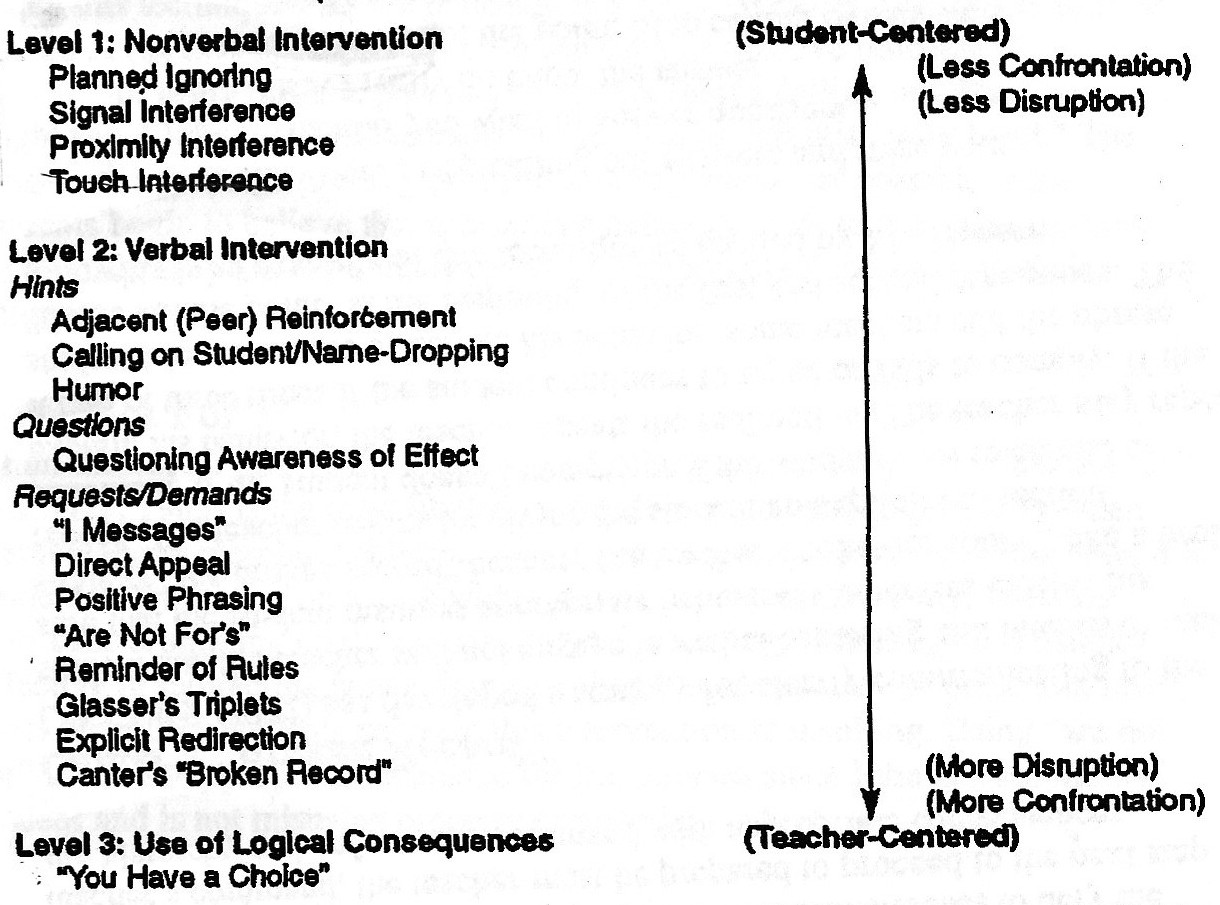
\includegraphics{./images/correctiveHierarchy.jpg}
\end{center}
\caption{Hierarchy of Management Intervention Diagram \cite{Levin2005} showing a list of corrective strategies, ranked in increasing order of harshness. Some of these are not applicable (such as touch), but many others on this list will be discussed in this chapter. \label{fig:correctiveHierarchy}}
\end{figure}


\section{Apply Sanctions}
\label{sec:sanctions_c}


\section{Give choice}
\label{sec:give choice_c}



\section{Arrange to talk privately with student about their misbehaviour}
\label{sec:private_talk_c}



\section{Use Names}
\label{sec:use_names_c}



\section{Show interest}
\label{sec:show_interest_c}


\section{Proximity ("The Whisper Technique")}
\label{sec:proximity_c}



\section{Eye Contact}
\label{sec:eye_contact_c}










\chapter{Video Examples}
\label{chap:video_examples}

Preparation (VIDEO: Praise and Preparation, Amy)

 Amy is a good example of structure this (VIDEO REFERENCE).

Non-verbals such as being happy to see the students (VIDEO: Talk too much).
A fantastic example of non-verbals this is simply being (genuinely) happy to see the students.
(VIDEO REFERENCE). Warning: Similar to with praise (\ref{sec:praise_p}), being genuine is crucial in this example --- if you are not genuine the students will be able to tell.



\chapter{Theories and Theorists}
\label{chap:theories}

Some theories I might want to discuss:
\begin{itemize}
  \item Cognitive Load Theory (CLT)
  \item Zone of Proximal Development (ZPD), Constructivism
  \item Operant Conditioning, Behaviourism
\end{itemize}



\bibliography{references}{}
\bibliographystyle{apalike}


\end{document}